\chapter{Antecedentes}
\label{cap:Antecedentes}
En este capítulo se introduce el contexto disciplinar y tecnológico en el que se desarrolla este trabajo.

\section{Herramientas de análisis de telemetría en Simracing}
En el mundo del Simracing, el análisis de telemetría se ha convertido en una herramienta esencial para mejorar el rendimiento y la comprensión del comportamiento del vehículo. Esta sección revisa algunas de las principales herramientas de análisis de telemetría disponibles para los entusiastas y profesionales del Simracing. Se destacan sus características, beneficios y cómo cada una contribuye al análisis detallado y preciso de los datos de telemetría.

\subsection{MoTec}
MoTec \cite{motec} es una herramienta avanzada de análisis de datos utilizada en diversas disciplinas del automovilismo. Permite a los usuarios visualizar y analizar datos de telemetría capturados durante las sesiones de conducción. Sus principales características incluyen gráficos superpuestos y en mosaico para comparar múltiples variables, soporte de cursores duales para mediciones diferenciales precisas, y sincronización automática de vídeo con datos registrados (\autoref{fig:motec}). Además, ofrece informes detallados en formatos tabulares y gráficos, y la capacidad de exportar datos en varios formatos como \ac{csv} y Matlab, facilitando un análisis profundo y exhaustivo de la telemetría del vehículo.
\begin{figure}[H]
	\centering
	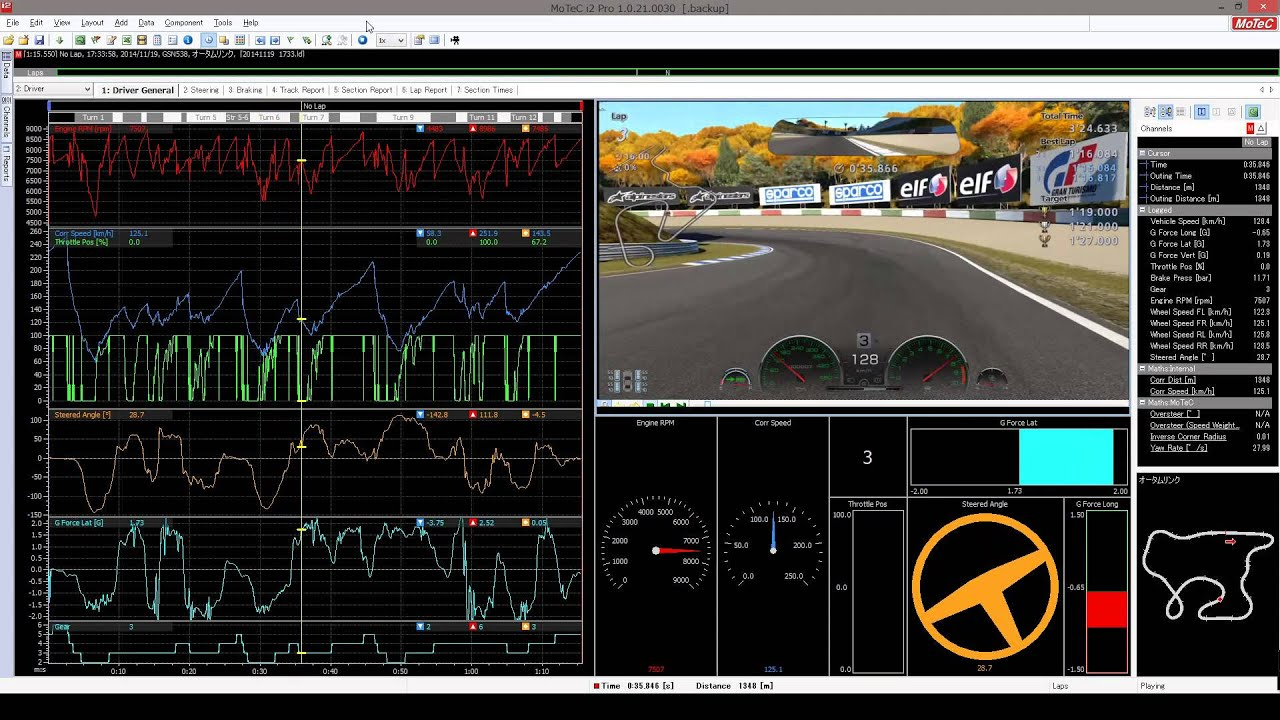
\includegraphics[width=0.6\linewidth]{./figs/herramientas/analisis/motec.png}
	\caption[Captura de Motec i2 Pro]{Captura de Motec i2 Pro \cite{motec_cap}}
    \label{fig:motec}
\end{figure}

\subsection{Mu}
Mu \cite{mu} es un exportador de telemetría que convierte los archivos de telemetría de iRacing (.ibt) en archivos que pueden ser leídos por el software i2 de MoTeC para su análisis. Entre sus características destacan la capacidad de exportar en formatos MoTeC y \ac{csv}, la exportación en unidades métricas o imperiales, y la activación automática de la captura de telemetría en iRacing. Además, Mu guarda una copia de la configuración utilizada para generar la telemetría y ofrece una interfaz de usuario que puede ejecutarse en segundo plano.

\subsection{McLaren Atlas}
McLaren Atlas \cite{atlas} es una herramienta de telemetría avanzada utilizada en competiciones de alto nivel como la Fórmula 1. Diseñada para proporcionar análisis detallados del rendimiento del vehículo (\autoref{fig:atlas}), Atlas permite a los ingenieros y pilotos comprender mejor el comportamiento del coche y optimizar su rendimiento. Sus características incluyen la capacidad de manejar grandes volúmenes de datos, realizar análisis detallados de cada componente del vehículo y generar informes claros que facilitan la interpretación de los datos y la implementación de mejoras específicas basadas en dichos análisis.

\begin{figure}[H]
	\centering
	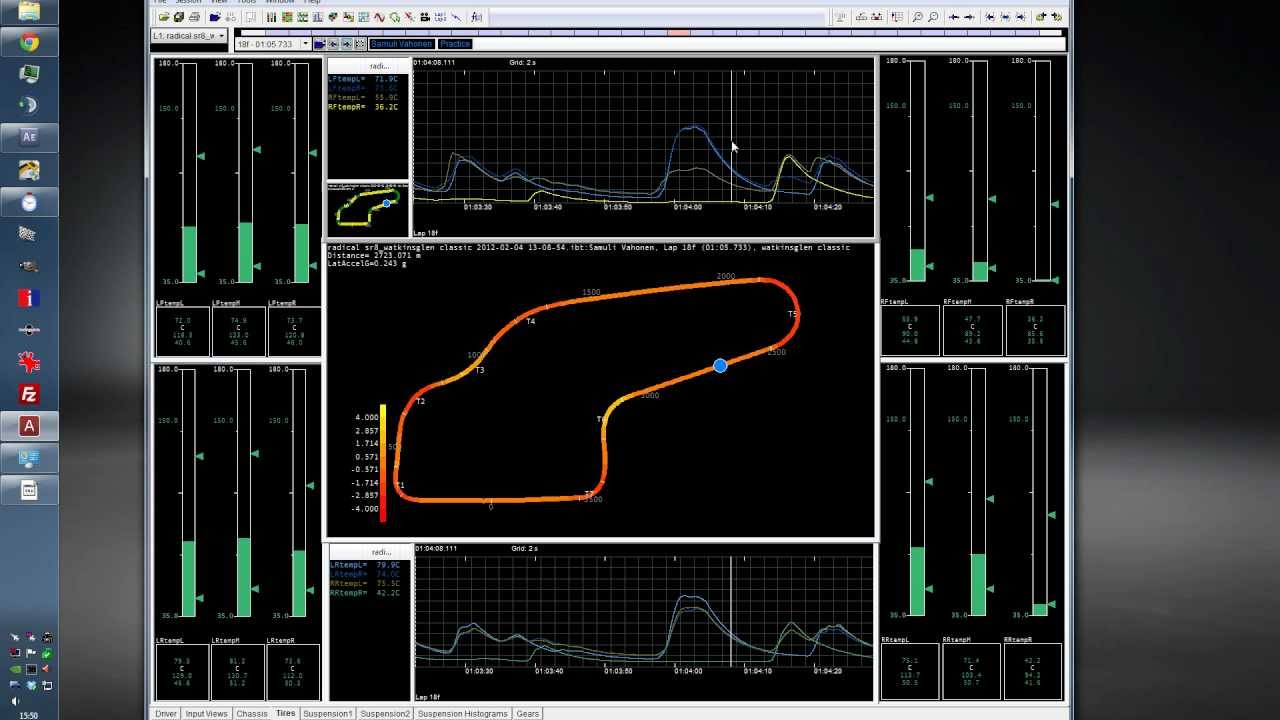
\includegraphics[width=0.6\linewidth]{./figs/herramientas/analisis/mclaren_atlas.png}
	\caption[Captura de McLaren Atlas]{Captura de McLaren Atlas \cite{atlas_cap}}
    \label{fig:atlas}
\end{figure}

\subsection{Sim Racing Telemetry}
Sim Racing Telemetry \cite{srt} es una herramienta versátil diseñada para el análisis de datos de telemetría en Simracing. Ofrece una interfaz amigable que permite a los usuarios importar datos de diversas plataformas de simulación y analizarlos mediante gráficos interactivos y comparaciones de vueltas (\autoref{fig:srt}). Entre sus características principales se incluyen la capacidad de comparar datos de múltiples sesiones, visualizar métricas clave en tiempo real y generar informes detallados. Esta herramienta es ideal tanto para aficionados como para profesionales que buscan mejorar su rendimiento en las simulaciones de carreras.
\begin{figure}[H]
	\centering
	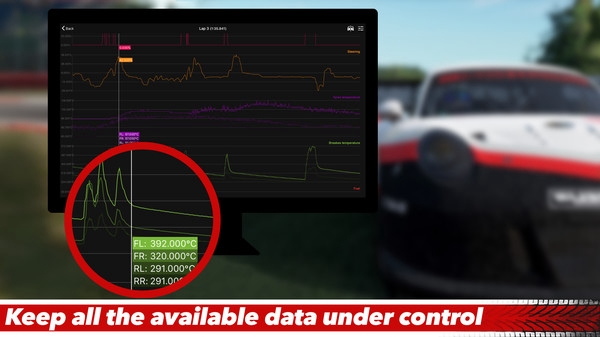
\includegraphics[width=0.6\linewidth]{./figs/herramientas/analisis/simracingtelemetry.png}
	\caption[Imagen promocional de Sim Racing Telemetry]{Imagen promocional de Sim Racing Telemetry \cite{srt_cap}}
    \label{fig:srt}
\end{figure}

\section{Entrenadores virtuales de Simracing}
En el Simracing, los entrenadores virtuales han revolucionado la forma en que los pilotos mejoran sus habilidades y estrategias de carrera. Estas herramientas proporcionan análisis detallados, asesoría personalizada y recursos educativos para ayudar a los simracers a alcanzar su máximo potencial. Esta sección explora algunos de los entrenadores virtuales más destacados, detallando sus características principales y cómo pueden beneficiar a los pilotos en su búsqueda de excelencia en las pistas virtuales.

\subsection{Virtual Racing School}
\ac{vrs} \cite{vrs} es una plataforma integral de entrenamiento que ofrece análisis de telemetría, tutoriales en vídeo, sesiones de entrenamiento en vivo con pilotos profesionales y programas de desarrollo personalizados. \ac{vrs} permite a los usuarios comparar sus datos con los de los mejores pilotos, identificar áreas de mejora y aplicar estrategias para optimizar su rendimiento en pista (\autoref{fig:vrs}). Además, proporciona recursos educativos a través de su academia en línea y soporte continuo para sus usuarios.
\begin{figure}[H]
	\centering
	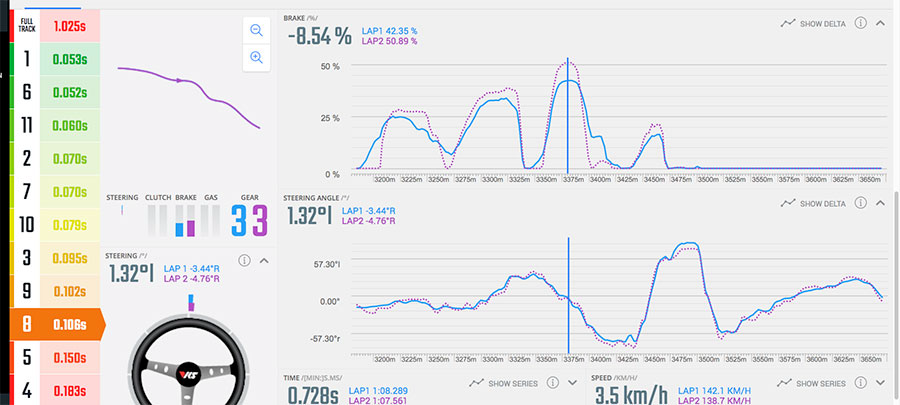
\includegraphics[width=0.6\linewidth]{./figs/herramientas/mentor_virtual/vrs.png}
	\caption[Imagen promocional de \ac{vrs}]{Imagen promocional de \ac{vrs} \cite{vrs_cap}}
    \label{fig:vrs}
\end{figure}

\subsection{Garage 61}
Garage 61 \cite{g61} es un servicio de mentoría personalizado para Simracers que se enfoca en el análisis detallado de telemetría, sesiones de práctica guiadas y retroalimentación en tiempo real (\autoref{fig:g61}). Las principales características de Garage 61 incluyen la adaptación de los programas de entrenamiento a las necesidades específicas de cada piloto y el acceso a un equipo de expertos en Simracing que ofrecen asesoramiento continuo. Esta plataforma ayuda a los pilotos a mejorar sus habilidades mediante un enfoque estructurado y personalizado.
\begin{figure}[H]
	\centering
	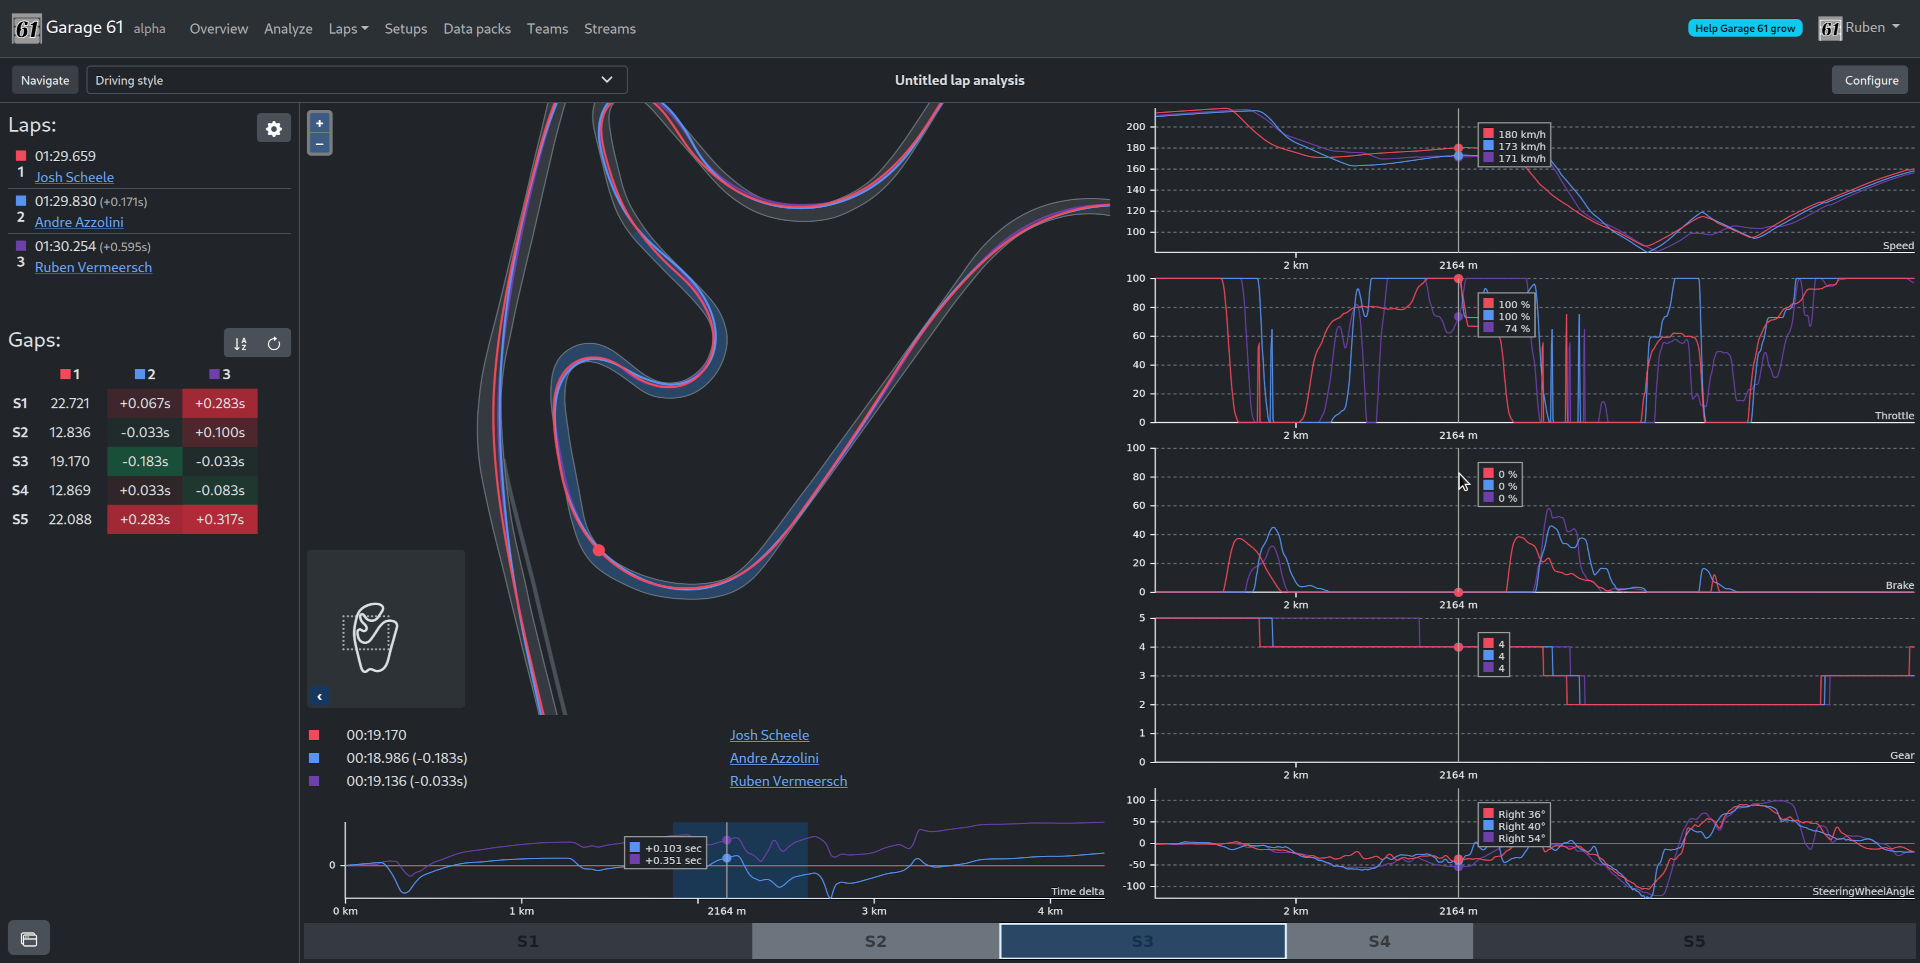
\includegraphics[width=0.6\linewidth]{./figs/herramientas/mentor_virtual/garage61.png}
	\caption[Imagen promocional de Garage 61]{Imagen promocional de Garage 61 \cite{g61_cap}}
    \label{fig:g61}
\end{figure}

\subsection{Grid-and-go Virtual Coach}
Grid-and-go Virtual Coach \cite{gg_vc} es una herramienta de mentoría en línea diseñada para mejorar el rendimiento de los Simracers mediante el análisis de datos y la asesoría personalizada (\autoref{fig:ggvc}). Ofrece una interfaz intuitiva para el análisis de telemetría, programas de entrenamiento estructurados y consejos estratégicos para la carrera. Entre sus características destacadas se encuentran la capacidad de establecer metas de rendimiento personalizadas, recibir recomendaciones basadas en datos y acceder a una comunidad de pilotos para compartir experiencias y estrategias.
\begin{figure}[H]
	\centering
	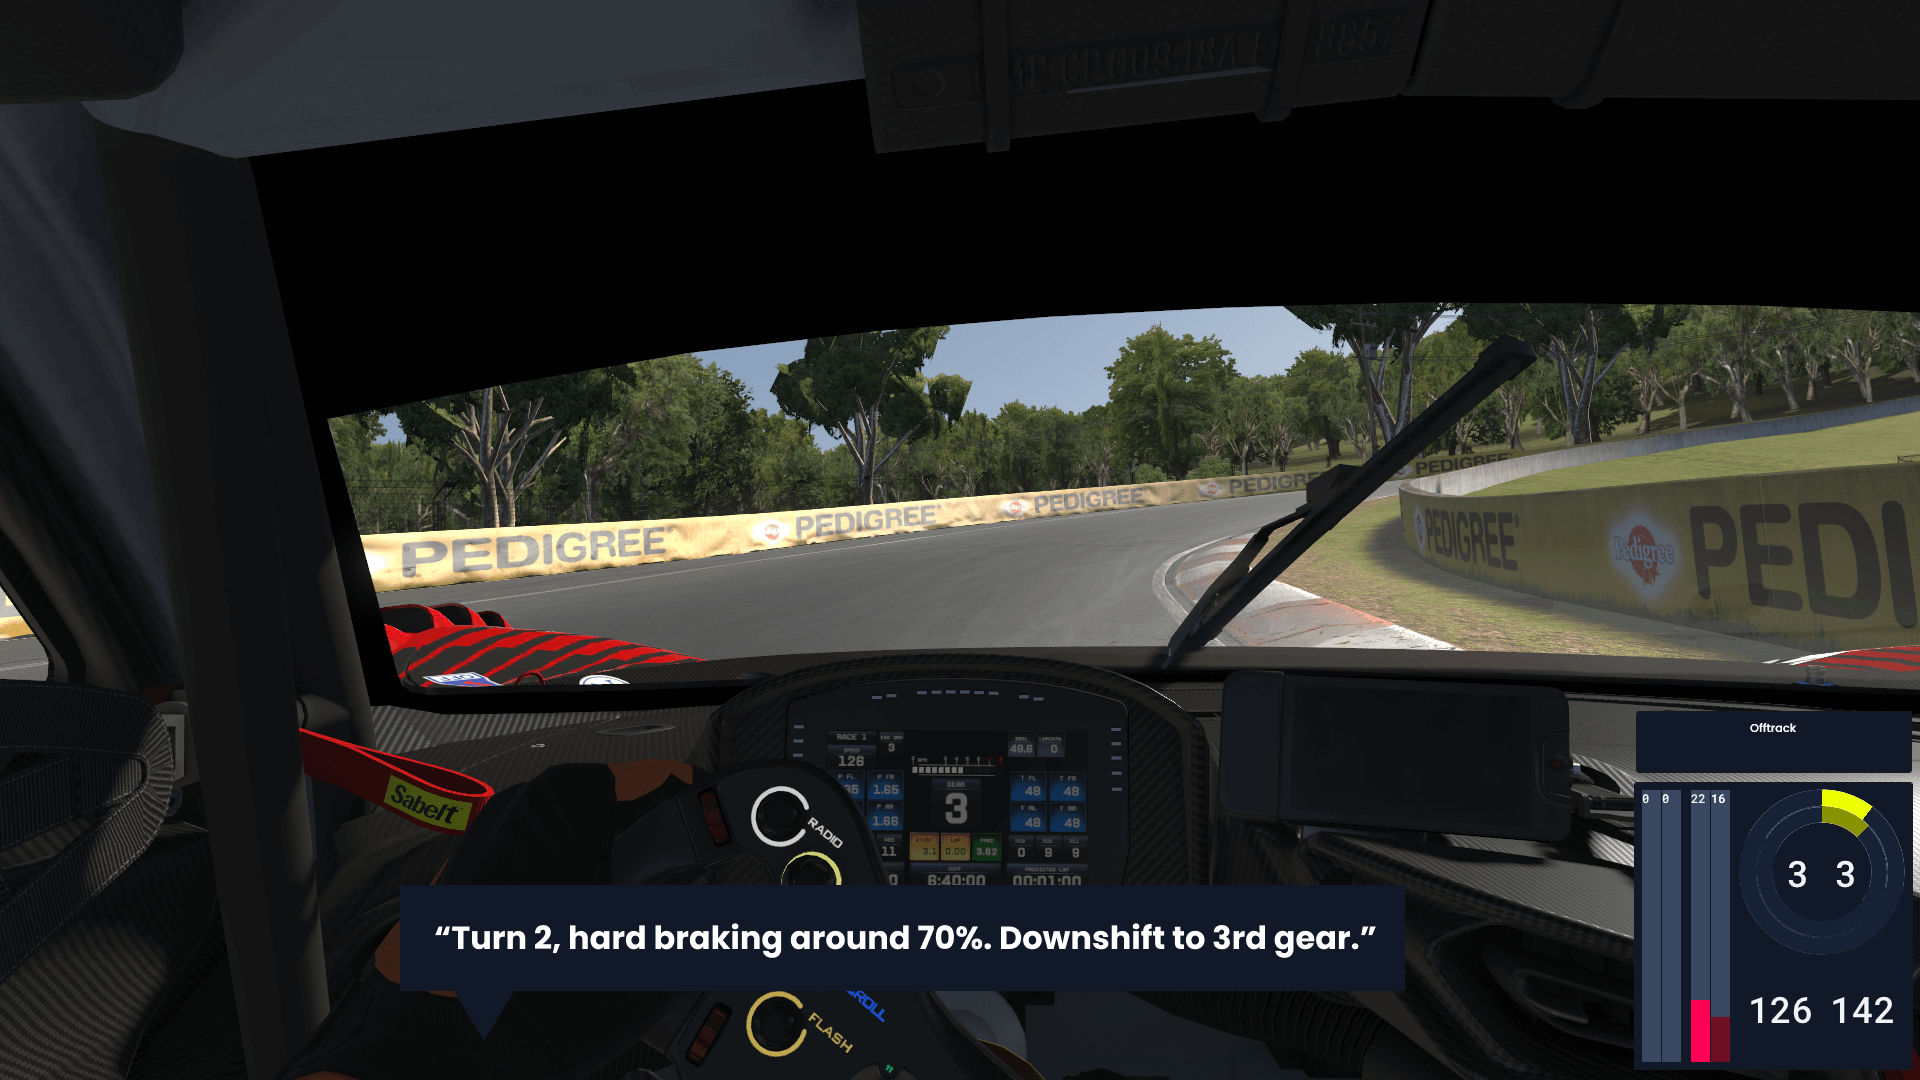
\includegraphics[width=0.6\linewidth]{./figs/herramientas/mentor_virtual/gg_virtual_coach.png}
	\caption[Imagen promocional de Grid-and-go Virtual Coach]{Imagen promocional de Grid-and-go Virtual Coach \cite{gg_vc_cap}}
    \label{fig:ggvc}
\end{figure}

\section{Repositorios abiertos de herramientas}
En el ámbito del Simracing, los repositorios abiertos de herramientas proporcionan a los desarrolladores y entusiastas la capacidad de personalizar y mejorar sus experiencias de simulación mediante el acceso a software y bibliotecas de código abierto. Estos recursos permiten la creación de aplicaciones avanzadas y la integración de funcionalidades adicionales que enriquecen el análisis y la práctica del Simracing. A continuación, se describen algunos de los repositorios más relevantes disponibles para la comunidad de Simracing.

\subsection{iRSDK}
iRSDK \cite{irsdk} es un clon del SDK oficial de iRacing en C++. Este repositorio proporciona una API limpia y ampliada que reemplaza la API de telemetría original de iRacing, soportando múltiples clientes y ofreciendo una lista expandida de funciones. iRSDK permite el acceso a datos de telemetría en tiempo real y la grabación de datos en disco, facilitando el desarrollo de aplicaciones que interactúan con la telemetría de iRacing para análisis y monitoreo en vivo.

\subsection{pyirsdk}
pyirsdk \cite{pyirsdk} es una implementación en Python 3 del SDK de iRacing. Este repositorio permite obtener datos de la sesión (como información del evento y de la sesión) y datos de telemetría en vivo, como velocidad y nivel de combustible. Además, soporta el envío de mensajes de difusión para controlar la cámara, reproducir repeticiones y ejecutar comandos durante el juego o mientras se permanece en el área de pit, zona de servicio y mantenimiento del vehículo. pyirsdk facilita la integración de la telemetría de iRacing en aplicaciones Python, proporcionando una herramienta poderosa y flexible para el análisis y el desarrollo en Simracing.

\subsection{itelem}
itelem \cite{itelem} es una herramienta de análisis de telemetría que convierte los archivos de telemetría de iRacing (.ibt) en un formato que puede ser utilizado para análisis detallado. Este repositorio permite a los usuarios desarrollar aplicaciones personalizadas para procesar y visualizar datos de telemetría, facilitando el estudio de diversos aspectos del rendimiento del vehículo y del piloto. Su diseño modular permite extensiones y adaptaciones según las necesidades específicas de los usuarios.

\subsection{ibt-telemetry}
ibt-telemetry \cite{ibt-telemetry} es una biblioteca destinada a la manipulación y análisis de archivos de telemetría .ibt de iRacing. Esta herramienta permite leer y procesar los datos almacenados en los archivos de telemetría, facilitando el desarrollo de aplicaciones que requieren acceso a información detallada de las sesiones de conducción. Con ibt-telemetry, los desarrolladores pueden extraer y analizar datos específicos para mejorar el rendimiento y la comprensión del comportamiento del vehículo en diferentes condiciones de carrera.

\section{Aprendizaje no supervisado}
El uso del aprendizaje automático, y en particular del aprendizaje no supervisado, ha demostrado ser fundamental en el análisis de datos complejos, como los que se generan en la telemetría de Simracing. Las técnicas de aprendizaje no supervisado, como el agrupamiento, permiten identificar patrones y asociar automáticamente datos similares sin necesidad de etiquetado previo \cite{Jain1988, Duda2000}. Esto es especialmente útil para categorizar vectores de diferencias en las variables de telemetría, facilitando la interpretación y el análisis de grandes volúmenes de datos. Al agrupar las diferencias en categorías significativas, estas técnicas proporcionan una visión más clara del rendimiento y comportamiento del vehículo y del piloto, permitiendo la optimización de estrategias de conducción basadas en datos precisos y categorizados\cite{Hastie2009, Bishop2006}.

\subsection{K-Means}
El algoritmo K-means es una técnica de aprendizaje no supervisado ampliamente utilizada para la agrupación de datos (\autoref{fig:km}). En el contexto del análisis de telemetría en Simracing, K-means es particularmente útil para categorizar las diferencias en las variables de telemetría, debido a su capacidad para minimizar la variabilidad dentro de los grupos y maximizar las diferencias entre ellos \cite{MacQueen1967}. Este proceso permite identificar patrones subyacentes en los datos de telemetría, facilitando la comprensión de las áreas donde se pueden realizar mejoras.

Una de las ventajas clave de utilizar K-means es que las categorías generadas tienden a estar ordenadas de manera natural. Esto significa que las diferencias en las variables de telemetría pueden agruparse en categorías jerárquicas, como ''muy poca diferencia negativa'', ''diferencia negativa'', ''igual'', ''diferencia positiva'' y ''mucha diferencia positiva''. Este ordenamiento facilita la asignación de etiquetas en lenguaje natural, lo que hace que los resultados sean fácilmente interpretables por los usuarios \cite{Jain1988, Hartigan1979}. Al proporcionar una descripción clara y ordenada de las diferencias, los pilotos pueden entender rápidamente las áreas que requieren atención y las acciones específicas que deben tomar para mejorar su rendimiento.

\begin{figure}[H]
	\centering
	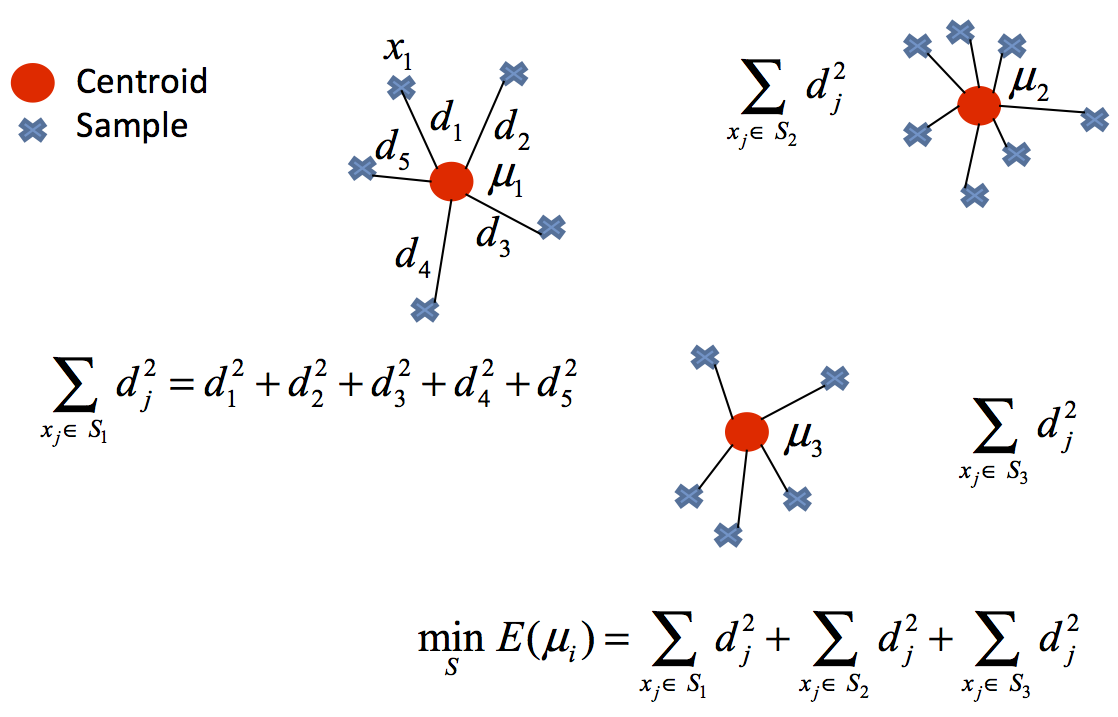
\includegraphics[width=0.6\linewidth]{./figs/aprendizaje_no_supervisado/k_means.png}
	\caption[Ilustración K-means (K = 3)]{Ilustración K-means (K = 3) \cite{UniOviedoKMeans}}
    \label{fig:km}
\end{figure}

\subsection{Fuzzy C-Means}

\ac{fcm} es un algoritmo de agrupamiento que permite que un punto de datos pertenezca a múltiples agrupaciones con diferentes grados de pertenencia (\autoref{fig:fcm}), en lugar de asignar cada punto a una sola agrupación de manera rígida. Esto se logra minimizando una función de costo que considera tanto la distancia entre los puntos de datos y los centroides de las agrupaciones como los grados de pertenencia \cite{Bezdek1981, Hathaway1996, Dunn1973, Pal1995}.

\begin{figure}[H]
	\centering
	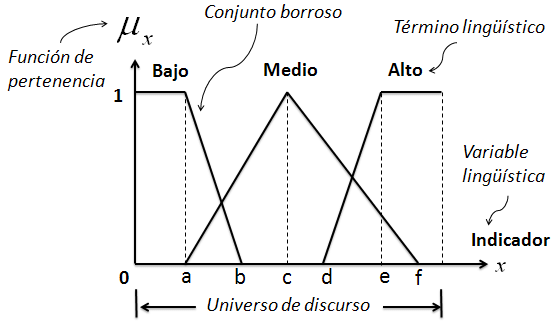
\includegraphics[width=0.6\linewidth]{./figs/aprendizaje_no_supervisado/conjuntos_borrosos.png}
	\caption[Ejemplo de conjuntos borrosos]{Ejemplo de conjuntos borrosos \cite{ResearchGateFuzzySets}}
    \label{fig:fcm}
\end{figure}

El algoritmo \ac{fcm} ofrece una mayor flexibilidad y precisión en la categorización de datos de telemetría en Simracing al permitir que cada punto de datos pertenezca a múltiples agrupaciones con diferentes grados de pertenencia. Esto facilita una interpretación más detallada y matizada, especialmente en presencia de ruido y ambigüedad en los datos. Los grados de pertenencia ayudan a generar etiquetas lingüísticas más comprensibles y graduales, mejorando la comprensión de los resultados. \ac{fcm} también es más adaptable a diferentes escenarios y condiciones cambiantes, proporcionando una herramienta versátil para el análisis de datos.